\documentclass[tikz,border=25pt]{standalone}
\usepackage{tikz}
\usetikzlibrary{shapes, arrows.meta, positioning, fit, backgrounds, calc, shadows}
\definecolor{acaBlueLine}{HTML}{6080B0}      \definecolor{acaBlueFill}{HTML}{DBEAFE}
\definecolor{acaGreenLine}{HTML}{30A060}     \definecolor{acaGreenFill}{HTML}{A0D0A0}
\definecolor{acaOrangeLine}{HTML}{D06020}    \definecolor{acaOrangeFill}{HTML}{FFE6CC}
\definecolor{acaPurpleLine}{HTML}{6020D0}    \definecolor{acaPurpleFill}{HTML}{E1D5E7}
\definecolor{acaGreyLine}{HTML}{666666}      \definecolor{acaGreyFill}{HTML}{F5F5F5}
\definecolor{acaGoldLine}{HTML}{D09000}
\definecolor{zoneGreenBg}{HTML}{ECFDF5}
\definecolor{zoneOrangeBg}{HTML}{FFF5EB}
\definecolor{zonePurpleBg}{HTML}{F5F3FF}
\pgfdeclarelayer{background}
\pgfsetlayers{background,main}
\begin{document}
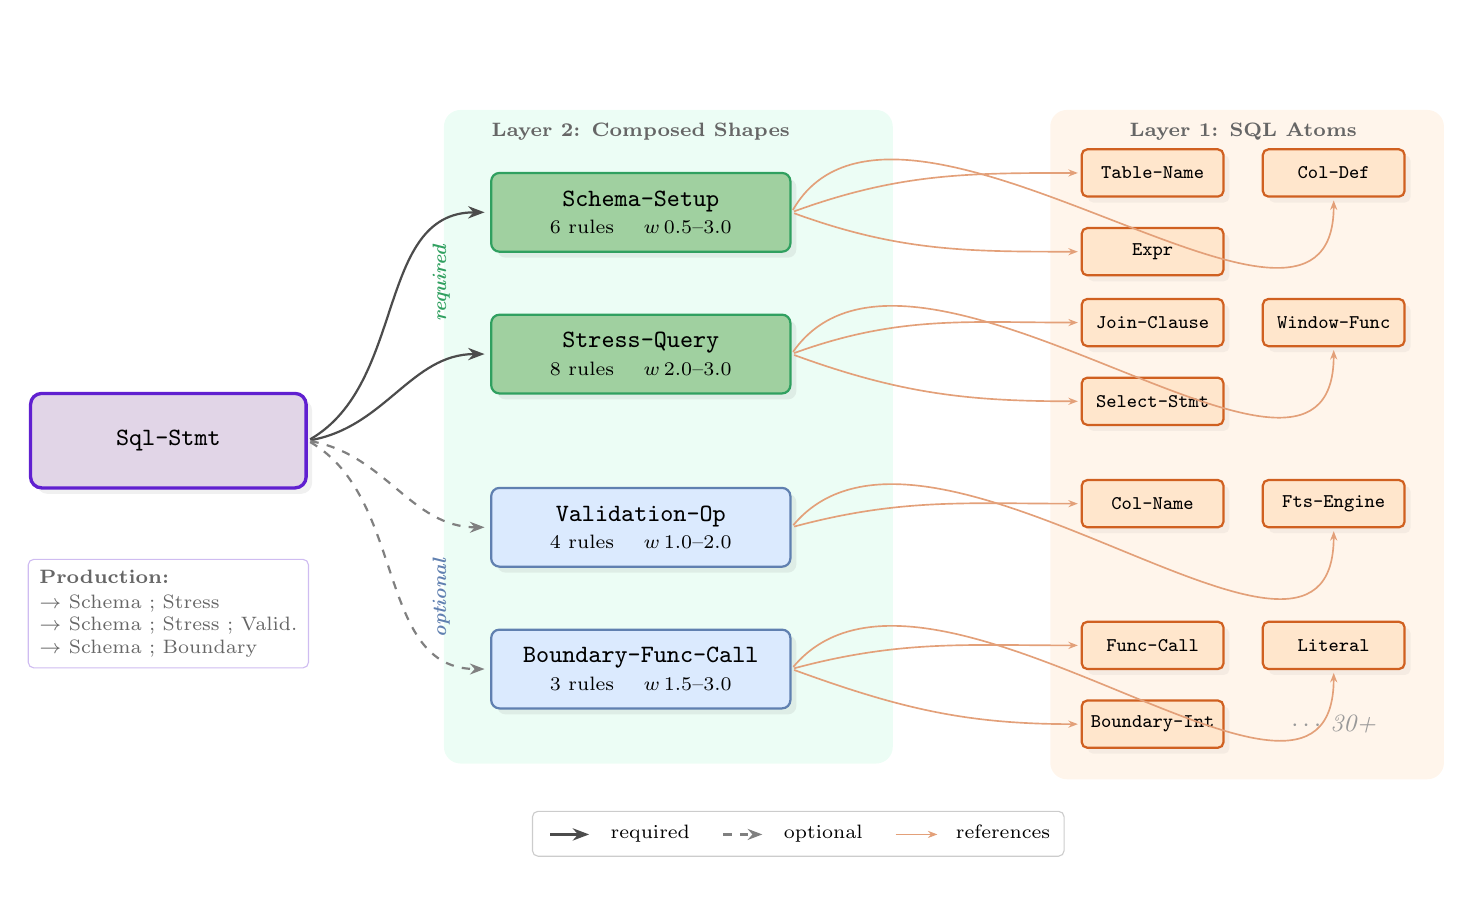
\begin{tikzpicture}[
    every node/.style={font=\small},
    rootbox/.style={rectangle, rounded corners=4pt, align=center,
        minimum width=3.5cm, minimum height=1.2cm,
        inner sep=8pt, very thick, draw=acaPurpleLine, fill=acaPurpleFill,
        drop shadow={opacity=0.12}, font=\small\bfseries},
    l2box/.style={rectangle, rounded corners=3pt, align=center,
        minimum width=3.8cm, minimum height=1.0cm,
        inner sep=6pt, thick, drop shadow={opacity=0.12}},
    l1box/.style={rectangle, rounded corners=2pt, align=center,
        minimum width=1.8cm, minimum height=0.6cm,
        inner sep=3pt, thick, font=\scriptsize,
        drop shadow={opacity=0.08}},
    arrow/.style={-{Stealth[scale=0.9]}, thick, color=black!70,
        shorten >=2pt, shorten <=1pt},
    dasharr/.style={-{Stealth[scale=0.8]}, thick, dashed, color=black!50,
        shorten >=2pt, shorten <=1pt},
    refarr/.style={-{Stealth[scale=0.6]}, semithick, color=acaOrangeLine!60,
        shorten >=1pt, shorten <=1pt},
    tag/.style={font=\scriptsize, inner sep=2pt},
    zonetag/.style={font=\scriptsize\bfseries, color=black!60, inner sep=3pt},
    wtag/.style={font=\tiny, color=acaGoldLine, inner sep=1pt},
]
    % ═══════════════════════════════════════════
    % COLUMN 1: Root — Sql-Stmt at vertical midpoint of L2 column
    % L2 spans y=3.2..9, so midpoint y=6.1
    % ═══════════════════════════════════════════
    \node[rootbox] (root) at (0, 6.1) {\texttt{Sql-Stmt}};
    % Composition rules just below the root (compact)
    \node[font=\scriptsize, color=black!60, align=left, anchor=north,
          draw=acaPurpleLine!30, rounded corners=2pt, fill=white,
          inner sep=4pt]
        at (0, 4.6) {
        \textbf{\scriptsize Production:}\\[1pt]
        $\to$ Schema ; Stress\\
        $\to$ Schema ; Stress ; Valid.\\
        $\to$ Schema ; Boundary
    };
    % ═══════════════════════════════════════════
    % COLUMN 2 (x=6): Layer 2 — Composed Shapes
    % ═══════════════════════════════════════════
    \node[l2box, fill=acaGreenFill, draw=acaGreenLine] (schema) at (6, 9) {
        \textbf{\texttt{Schema-Setup}}\\[-1pt]
        {\scriptsize 6 rules \quad $w$\,0.5--3.0}
    };
    \node[l2box, fill=acaGreenFill, draw=acaGreenLine] (stress) at (6, 7.2) {
        \textbf{\texttt{Stress-Query}}\\[-1pt]
        {\scriptsize 8 rules \quad $w$\,2.0--3.0}
    };
    \node[l2box, fill=acaBlueFill, draw=acaBlueLine] (valid) at (6, 5.0) {
        \textbf{\texttt{Validation-Op}}\\[-1pt]
        {\scriptsize 4 rules \quad $w$\,1.0--2.0}
    };
    \node[l2box, fill=acaBlueFill, draw=acaBlueLine] (boundary) at (6, 3.2) {
        \textbf{\texttt{Boundary-Func-Call}}\\[-1pt]
        {\scriptsize 3 rules \quad $w$\,1.5--3.0}
    };
    % Required / Optional brace labels (vertical, on the left edge of L2 zone)
    \node[font=\scriptsize\bfseries\itshape, color=acaGreenLine, rotate=90, anchor=south]
        at (3.7, 8.1) {required};
    \node[font=\scriptsize\bfseries\itshape, color=acaBlueLine, rotate=90, anchor=south]
        at (3.7, 4.1) {optional};
    % ═══════════════════════════════════════════
    % COLUMN 3 (x=12.5/14.8): Layer 1 — SQL Atoms
    % Atom y-coords kept matching their primary L2's vertical band
    % ═══════════════════════════════════════════
    % Schema atoms (y around 9)
    \node[l1box, fill=acaOrangeFill, draw=acaOrangeLine] (tname) at (12.5, 9.5) {\texttt{Table-Name}};
    \node[l1box, fill=acaOrangeFill, draw=acaOrangeLine] (coldef) at (14.8, 9.5) {\texttt{Col-Def}};
    \node[l1box, fill=acaOrangeFill, draw=acaOrangeLine] (expr) at (12.5, 8.5) {\texttt{Expr}};
    % Stress atoms (y around 7.2)
    \node[l1box, fill=acaOrangeFill, draw=acaOrangeLine] (joinc) at (12.5, 7.6) {\texttt{Join-Clause}};
    \node[l1box, fill=acaOrangeFill, draw=acaOrangeLine] (winfunc) at (14.8, 7.6) {\texttt{Window-Func}};
    \node[l1box, fill=acaOrangeFill, draw=acaOrangeLine] (selectst) at (12.5, 6.6) {\texttt{Select-Stmt}};
    % Validation atoms (y around 5.0)
    \node[l1box, fill=acaOrangeFill, draw=acaOrangeLine] (colname) at (12.5, 5.3) {\texttt{Col-Name}};
    \node[l1box, fill=acaOrangeFill, draw=acaOrangeLine] (ftseng) at (14.8, 5.3) {\texttt{Fts-Engine}};
    % Boundary atoms (y around 3.2)
    \node[l1box, fill=acaOrangeFill, draw=acaOrangeLine] (funccall) at (12.5, 3.5) {\texttt{Func-Call}};
    \node[l1box, fill=acaOrangeFill, draw=acaOrangeLine] (literal) at (14.8, 3.5) {\texttt{Literal}};
    \node[l1box, fill=acaOrangeFill, draw=acaOrangeLine] (boundint) at (12.5, 2.5) {\texttt{Boundary-Int}};
    \node[font=\small\itshape, color=black!40] at (14.8, 2.5) {$\cdots$ 30+};
    % ═══════════════════════════════════════════
    % ARROWS: Root → L2  — proper FAN-OUT using out/in angles
    % All arrows leave from root.east at different vertical points
    % and enter their target's west at a horizontal angle (180°)
    % ═══════════════════════════════════════════
    % Required (solid) — schema (up) and stress (slightly up)
    \draw[arrow] (root.east) to[out=30, in=180] (schema.west);
    \draw[arrow] (root.east) to[out=10, in=180] (stress.west);
    % Optional (dashed) — valid (slightly down) and boundary (down)
    \draw[dasharr] (root.east) to[out=-10, in=180] (valid.west);
    \draw[dasharr] (root.east) to[out=-30, in=180] (boundary.west);
    % ═══════════════════════════════════════════
    % ARROWS: L2 → L1 references
    % Each L2 fans out to its atoms using out/in angles
    % Enter atoms from the LEFT (in=180), leave L2 from the right (out=...)
    % Tune out-angles based on whether atom is above/below/level with L2
    % ═══════════════════════════════════════════
    % Col-1 atoms (x=12.5) enter from WEST (left).
    % Col-2 atoms (x=14.8) enter from SOUTH (bottom) so the line goes
    % up-and-over above the col-1 atom and drops cleanly onto col-2.
    % --- Schema-Setup (y=9) → tname (col1,9.5), coldef (col2,9.5), expr (col1,8.5)
    \draw[refarr] (schema.east) to[out=20,  in=180] (tname.west);
    \draw[refarr] (schema.east) to[out=60,  in=270] (coldef.south);
    \draw[refarr] (schema.east) to[out=-20, in=180] (expr.west);
    % --- Stress-Query (y=7.2) → joinc (col1,7.6), winfunc (col2,7.6), selectst (col1,6.6)
    \draw[refarr] (stress.east) to[out=20,  in=180] (joinc.west);
    \draw[refarr] (stress.east) to[out=55,  in=270] (winfunc.south);
    \draw[refarr] (stress.east) to[out=-20, in=180] (selectst.west);
    % --- Validation-Op (y=5.0) → colname (col1,5.3), ftseng (col2,5.3)
    \draw[refarr] (valid.east)  to[out=15,  in=180] (colname.west);
    \draw[refarr] (valid.east)  to[out=50,  in=270] (ftseng.south);
    % --- Boundary-Func-Call (y=3.2) → funccall (col1,3.5), literal (col2,3.5), boundint (col1,2.5)
    \draw[refarr] (boundary.east) to[out=15,  in=180] (funccall.west);
    \draw[refarr] (boundary.east) to[out=50,  in=270] (literal.south);
    \draw[refarr] (boundary.east) to[out=-20, in=180] (boundint.west);
    % ═══════════════════════════════════════════
    % ZONE BACKGROUNDS
    % ═══════════════════════════════════════════
    \begin{pgfonlayer}{background}
        \fill[zoneGreenBg, rounded corners=6pt]
            (3.5, 2.0) rectangle (9.2, 10.3);
        \fill[zoneOrangeBg, rounded corners=6pt]
            (11.2, 1.8) rectangle (16.2, 10.3);
    \end{pgfonlayer}
    % Place zone titles at TOP-CENTER, above the highest L2/L1 nodes
    \node[zonetag, anchor=north] at (6.0, 10.25) {Layer 2: Composed Shapes};
    \node[zonetag, anchor=north] at (13.65, 10.25) {Layer 1: SQL Atoms};
    % ═══════════════════════════════════════════
    % LEGEND (bottom)
    % ═══════════════════════════════════════════
    \node[font=\scriptsize, anchor=north,
          draw=black!20, rounded corners=2pt, fill=white, inner sep=5pt]
        at (8.0, 1.4) {
        \tikz[baseline=-0.5ex] \draw[arrow] (0,0) -- (0.6,0);
        ~required \quad
        \tikz[baseline=-0.5ex] \draw[dasharr] (0,0) -- (0.6,0);
        ~optional \quad
        \tikz[baseline=-0.5ex] \draw[refarr] (0,0) -- (0.6,0);
        ~references
    };
\end{tikzpicture}
\end{document}